\documentclass{scrreprt}
\usepackage{listings}
\usepackage{underscore}
\usepackage[bookmarks=true]{hyperref}
\usepackage[utf8]{inputenc}
\usepackage[english]{babel}
\usepackage{glossaries}
\usepackage{graphicx}
\usepackage{caption}
\usepackage{flafter}
\usepackage{enumitem}
\usepackage{float}
\hyphenpenalty=10000
\date{}
\usepackage{hyperref}
\addto\captionsenglish{
  \renewcommand{\contentsname}
    {Table of Contents}
}
\begin{document}

\begin{flushright}
    \rule{16cm}{5pt}\vskip1cm
    \begin{bfseries}
        \Huge{SOFTWARE REQUIREMENTS\\ SPECIFICATION}\\
        \vspace{1.9cm}
        for\\
        \vspace{1.9cm}
        Donors Choose\\
        \vspace{1.9cm}
        \LARGE{Version 1.0}\\
        \vspace{1.9cm}
        Prepared by\\
        Fida Kamal (180041208)\\
        Fariha Fairoz Nohan (180041214)\\
        Alvi Aveen Khan (180041229)\\
        \vspace{1.9cm}
        \today\\
    \end{bfseries}
\end{flushright}

\tableofcontents

\chapter{Introduction}

\section{Purpose}
The purpose of this document is to detail the software requirements for a Donation Management System. It will describe details of the different features that will be implemented in the system and how users can interact with the system.\\

\section{Intended Audience}

This document is intended for both stakeholders and developers of the system, as well as any supervisors overlooking the development team.\\

\section{Project Scope}

The system will be available to potential donors to make the process of donating to the range of charities available in Bangladesh more comfortable for them while at the same time making the overall process of donating more effective. It will provide them with features to search for information about charities, stay up-to-date about their activities, make donations and receive updates about their donations.\\

The system will also be available to charities and will work as a platform to expand their reach. They will be able to provide details about their activities to users, provide donation updates to donors and receive information about users interested in donating to them.\\

\chapter{Overall Description}

\section{Product Perspective}

The system will act as a medium between potential donors and charities.\\

Potential donors will be able to search for charities and even for different categories of donations upon which they will be shown a range of choices. On the page for a specific charity, they will be able to see a general overview of the charity, as well as the different activities currently underway. They will have the option to provide details to the charity for collection of non-monetary donations or provide monetary donations directly through their bank accounts.\\

Charity organizations will be able to inform potential donors about the activities they are partaking in, collect information about donors who are willing to make non-monetary donations and inform past donors about the outcomes of their donations. The charities will have to contact support staff and verify that they are a legitimate non-profit organization, upon which they will be given an account on the system.\\


\section{Product Functions}

Donors will be able to
\begin{itemize}
  \item Register for a profile
  \item Search for information regarding charities
  \item Stay up-to-date about their favorite charities
  \item Donate to their desired charities
  \item Receive updates about previous donations
  \item Leave reviews for charities they have donated to\\
\end{itemize}
\clearpage
Charities will be able to
\begin{itemize}
  \item Keep information about their organization and their activities on their homepage
  \item Highlight activities on the homepage of any donors interested in the organization
  \item Update past donors about the status of their donations
  \item Collect information about potential donations\\
\end{itemize}

\section{User Classes and Characteristics}

The system divides its users into two categories, donors and charity organizations.\\

Donors can be anyone looking to make donations or learn more about charities available in the country. The system will be designed to accommodate anyone with or without any technical competency. All the different features should be prominently displayed and easy to use. Individual users of this category may or may not use the system frequently.\\

Charity organizations will have profiles within the system that donors will be able to view. It is expected that these profiles will be managed by appointed representatives of the charity organizations. They should have experience with managing the profile just as they would do for a social media platform. Extensive guidance regarding the management of charity profiles will not be provided by the system or by any support staff. They are also expected to frequently use the system so as to manage any requests for non-monetary donations by donors.\\


\section{Operating Environment}

The software will be able to operate on any computer running on the Windows operating system or any emulator running the Windows operating system.\\

\section{Design and Implementation Constraints}

The development of the payment gateway for transactions for monetary donations is limited to the existing, secure gateways. A custom gateway will not be built for the system under any circumstances due to the security risks involved.\\

With regards to time, the development team will only have until the first week of January, 2020 to develop the system. This might cause some features that are determined to be of lesser importance to be dropped.\\

\section{Assumptions and Dependencies}

The feature to notify users about the outcomes of donations is based on the assumption that charities will provide such updates regularly. If charities fail to provide such updates, this feature will not work as intended.\\

On the software side, it is assumed that a server-side database will not be available for now. As such, the current system is being developed on SQLite and being synced with an online cloud storage manually. If a server-side database becomes available for use, there will likely be changes to the amount of network bandwidth on the user side required by the system.\\


\chapter{External Interface Requirements}

\section{User Interfaces}

When the system is started by the user, a registration and login page will be shown where they can register/login using a unique username and password. There will be a warning to make sure their username is memorable, since no account recovery process will be available for now. In the registration process, if the username is not unique, an error message will be shown informing the user about this. In the login process, if the login credentials are incorrect, an error message will be shown to inform the user.\\

After the login process is complete, the interface is divided into two categories, one for donors and one for representatives of charity organizations.\\

\subsection*{User Interface for Donors}

Once logged in, the user will be taken to their homepage. There will be a navigation menu with options to go to different parts of the system. This navigation menu will be available everywhere on the program except for the on the payment gateway when making monetary transactions.\\

The homepage itself will consist of short descriptions of the activities of the highest rated charities in the system. There will also be a search bar at the top. Users will be able to use this search to search for different charities and categories of donations. A list of results will be shown when a search is made. Users can choose a result from this list, upon which they will be taken to the profile page of the relevant charity.\\

The profile page of the charity will consist of details about the charity, their recent activities and an option to donate to the charity. Choosing to donate will give the user two options, either for a monetary donation or for a non-monetary donation.\\

Choosing to make a monetary donation will take the user to a form which will prominently display information about the charity and its bank account information. There will be a field where the user will enter the amount they want to donate. Upon confirming this amount, the user will be taken to a payment gateway. This gateway will not be designed by the development team due to security concerns. An existing, secure gateway will be used instead.\\

Choosing to make a non-monetary donation will take the user to a form where they can provide information about what they want to donate as well as personal information such as their name, contact number or email. They must also provide a pickup point from where a representative of the charity will be expected to meet the donor to receive their donation. This can be at the office of the charity if the donor wishes to go there.\\

After either type of donation is complete, the user will be shown a confirmation message.\\

From the navigation menu, the user will be able to access their own profile. Here, they will simply be shown the option to change their password. No other information about the user will be stored by the system. There will also be a list of past donations made by the user on this page. They will have the option to leave reviews they have donated to in the past in the form of a rating.\\

\subsection*{User Interface for Charities}

If a representative of the charity is logging in, they will see a profile page for their charity. If this is the first time they are logging in, then they must provide some basic information about the charity such as the name and description. They must also provide some contact information such as an email address.\\

There will be an option to add new activities. The interface for this will be a form where different details about the activity can be added.\\

\subsection*{General User Interface}

A logout option will be available to both categories of users in the navigation menu.\\

The interface will remain simple throughout, since the system is not meant for technically competent users. All instructions will be prominently displayed so that the system is usable by anyone with the least past experience with a computer. Any error messages shown to users will be informative and make it clear what needs to be fixed.\\


\section{Hardware Interfaces}

The only end-user devices currently supported by the system are personal computers running the Windows operating system. An internet connection, either wired or wireless, is required. However, the system will not be network intensive.\\

\section{Software Interfaces}

There are two interactions that occur between the system and entities outside the system.\\

The first is with banks. When making monetary donations, donors must provide transaction information. This information will be collected using a payment gateway. This payment gateway will not be developed by the development team due to security concerns. Instead, an existing, secure gateway will be used. The transaction information will be delivered to the relevant bank for verification by the gateway.\\

The second is with an online cloud storage where the database will be stored. The entire database will be stored locally and be synchronized with the cloud storage. The synchronization process will take place when the system first starts up and also after any changes are made to any piece of data by the user. This includes changes to login information, changes to the details or activities of charities by representatives and any donations made by donors.\\

\section{Communications Interfaces}

The system will use an online cloud storage API to synchronize the local database.

\chapter{System Features}

\section{Making Donations}

\vspace{1cm}

\subsection{Description and Priority}

Donors will be able to make monetary and non-monetary donations to any charity of their choice from the charity profile page. This is a High priority feature.\\

\subsection{Stimulus/Response Sequences}

\begin{enumerate}[label=(\alph*)]
\item The donor will register or login.
\item The donor will search for a charity or for a donation category. The system will respond by providing a list of possible results.
\item The donor will select a specific charity from the list of results. The system will respond by displaying the profile page of the charity.
\item The donor will be able to select an option to make a monetary or a non-monetary donation on the charity profile page. They will also be able to specify if they wish to donate to a particular activity. The system will respond to a monetary donation request by taking the user to the payment gateway. The system will respond to a non-monetary donation request by taking the user to a form where they can provide information regarding the donation.
\item For monetary donations, the payment gateway will handle the actual transaction process. An existing, secure gateway will be used for this purpose.
\item For non-monetary donations, the donor will have to fill out the form provided to them. The system will then deliver the information provided by the user to the respective charity.\\

\end{enumerate}

\clearpage

\subsection{Functional Requirements}

REQ-1:	A database must be maintained to verify the donor’s login information. Incorrect information will be met with an error message describing the problem.\\
\\REQ-2:	A database must be maintained to store details about the different charities. Searches that do not match any results will be met with a message informing the user that there were no results.\\
\\REQ-3:	A existing, secure payment gateway will be used to handle monetary donations. It must be ensured that the gateway handles incorrect transaction details properly. The details about this have not yet been decided.\\
\\REQ-4:	The form used for non-monetary donations will highlight fields that are required and cannot be left empty. Appropriate error messages will be shown if required information is left out.\\


\section{Donation Updates}

\vspace{1cm}

\subsection{Description and Priority}

Charities will be able to provide updates about donations made by donors in the past. Donors will receive such updates in the form of a notification. Only donors that have specified which activity they are donating to will receive such a notification. Those who made general donations without specifying an activity will not. This feature has a Medium priority.\\

\subsection{Stimulus/Response Sequences}

\begin{enumerate}[label=(\alph*)]
\item A user logged in to a charity organization account will be able to update an existing activity.
\item The system will search through the database for donations made to that particular activity.
\item The system will send a notification to any users that have donated to that activity informing them about the update made to the activity.\\

\end{enumerate}

\subsection{Functional Requirements}

REQ-1:	A database must be maintained to store the different activities of the charities.\\
\\REQ-2:	A database must be maintained to store the details of the different donations, including details about which donors made the donations and which activities they donated to.\\


\section{Review Charities}

\vspace{1cm}

\subsection{Description and Priority}

Donors will be able to leave reviews for charities they have donated to. This is a Medium priority feature.\\

\subsection{Stimulus/Response Sequences}

\begin{enumerate}[label=(\alph*)]
\item A user logged in to a donor account will be able to access their profile page from the navigation menu. The profile page will contain a list of donations made by the donor. The system will retrieve the data for this list when the user accesses this page.
\item Along with every donation entry, there will be an option to leave a rating for the charity. If the user provides a rating next to a donation entry, the system will recalculate the average rating for that charity and store it with the information regarding the charity in the database.\\

\end{enumerate}

\subsection{Functional Requirements}

REQ-1:	A database must be maintained to store the details of the different charities, including their average rating calculate from the reviews left by all donors.\\


\chapter{Other Nonfunctional Requirements}

\section{Performance Requirements}

The only performance requirements relate to the database being used. As specified earlier, no server-side database is currently available for the system. A local database must be used and synchronized manually. The database must be synchronized every time there are changes to data being stored in the database, such as when a charity makes any changes to their profile or when a donor makes a donation, so as to ensure the most up-to-date version of the database is available in the online storage.\\

\section{Security Requirements}

The system will not store any personal information about donors. The only information that will be stored will be their login information and their donation history.\\

The system will only store official contact information about charities as well as information about bank accounts to allow for monetary donations.\\

Except for passwords, none of the other data raises concerns about privacy or security. Password must use at least a minimal level of encryption.\\

The database should be kept as lightweight as possible so as to reduce network bandwidth requirements on the user’s side.\\

Regarding monetary donations, the system must use a secure payment gateway. An existing gateway will be used for this purpose due to the security risks involved. The system should not attempt to access any transaction information of donors. The entire transaction process is to be managed by the gateway.\\


\section{Software Quality Attributes}

The system must be designed in a simple manner that would be easy to understand from the perspective of users with the least technical competency.\\

\section{Business Rules}

Profiles for charity organizations cannot be setup through the registration process available in the system. A representative from the charity will have to contact support staff in order to verify the legitimacy of the organization. Once this is done, they will be provided with login information for a blank profile for their charity.\\

\addchap{Appendix A: Glossary}

\subsection*{Charity}
A charity, charity organization, or representative of a charity organization refers to a user that is logged into the system after have requested and received a public charity profile. These are users that will be able to edit information on the profile page for the charity they are registered as. They will not have access to the other parts of the system.\\

\subsection*{Donor}
A donor is a user that has logged into the system after having register for a private profile. These are the users that will be able to view charity profiles and make donations to them.\\

\addchap{Appendix B: Analysis Models}

\begin{figure}[!h]
    \centering
    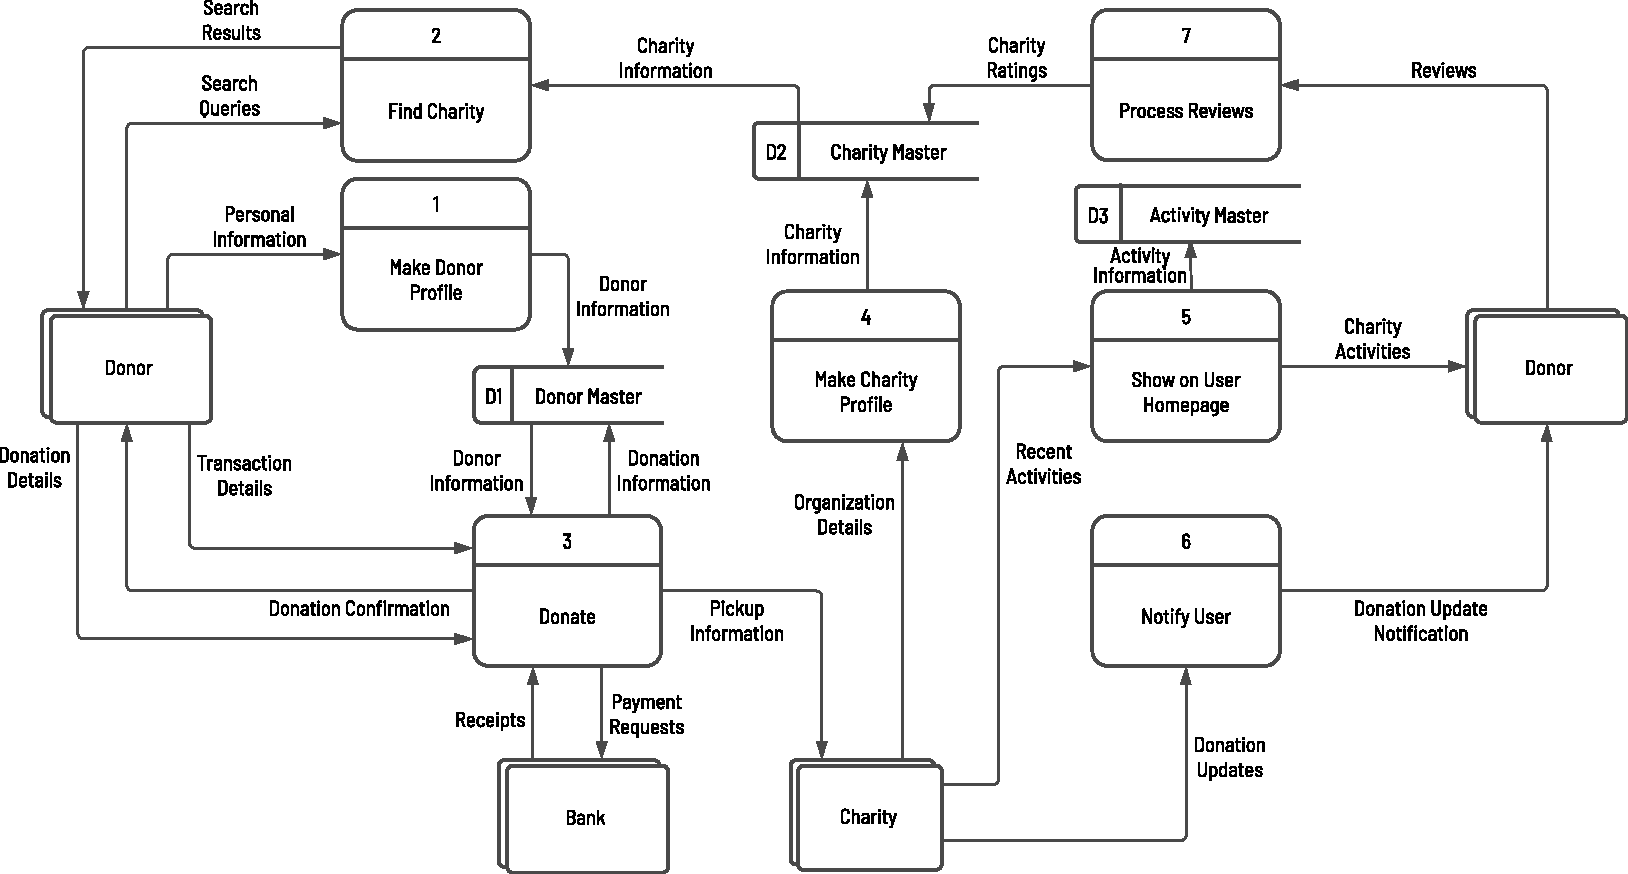
\includegraphics[width=0.90\linewidth]{Diagram 0.png}
    {\caption*{Data Flow Diagram - Diagram 0}}
\end{figure}

\vspace{1cm}

\begin{figure}[!h]
    \centering
    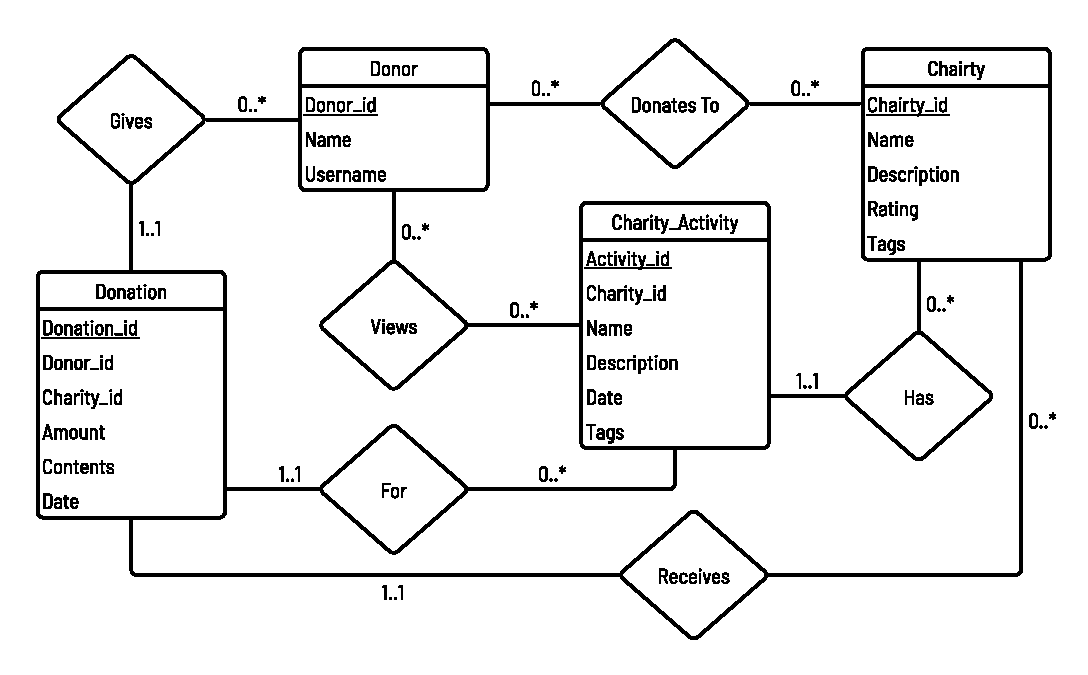
\includegraphics[width=0.65\linewidth]{ER Diagram.png}
    {\caption*{Entity-Relationship Diagram}}
\end{figure}

\begin{figure}[H]
    \centering
    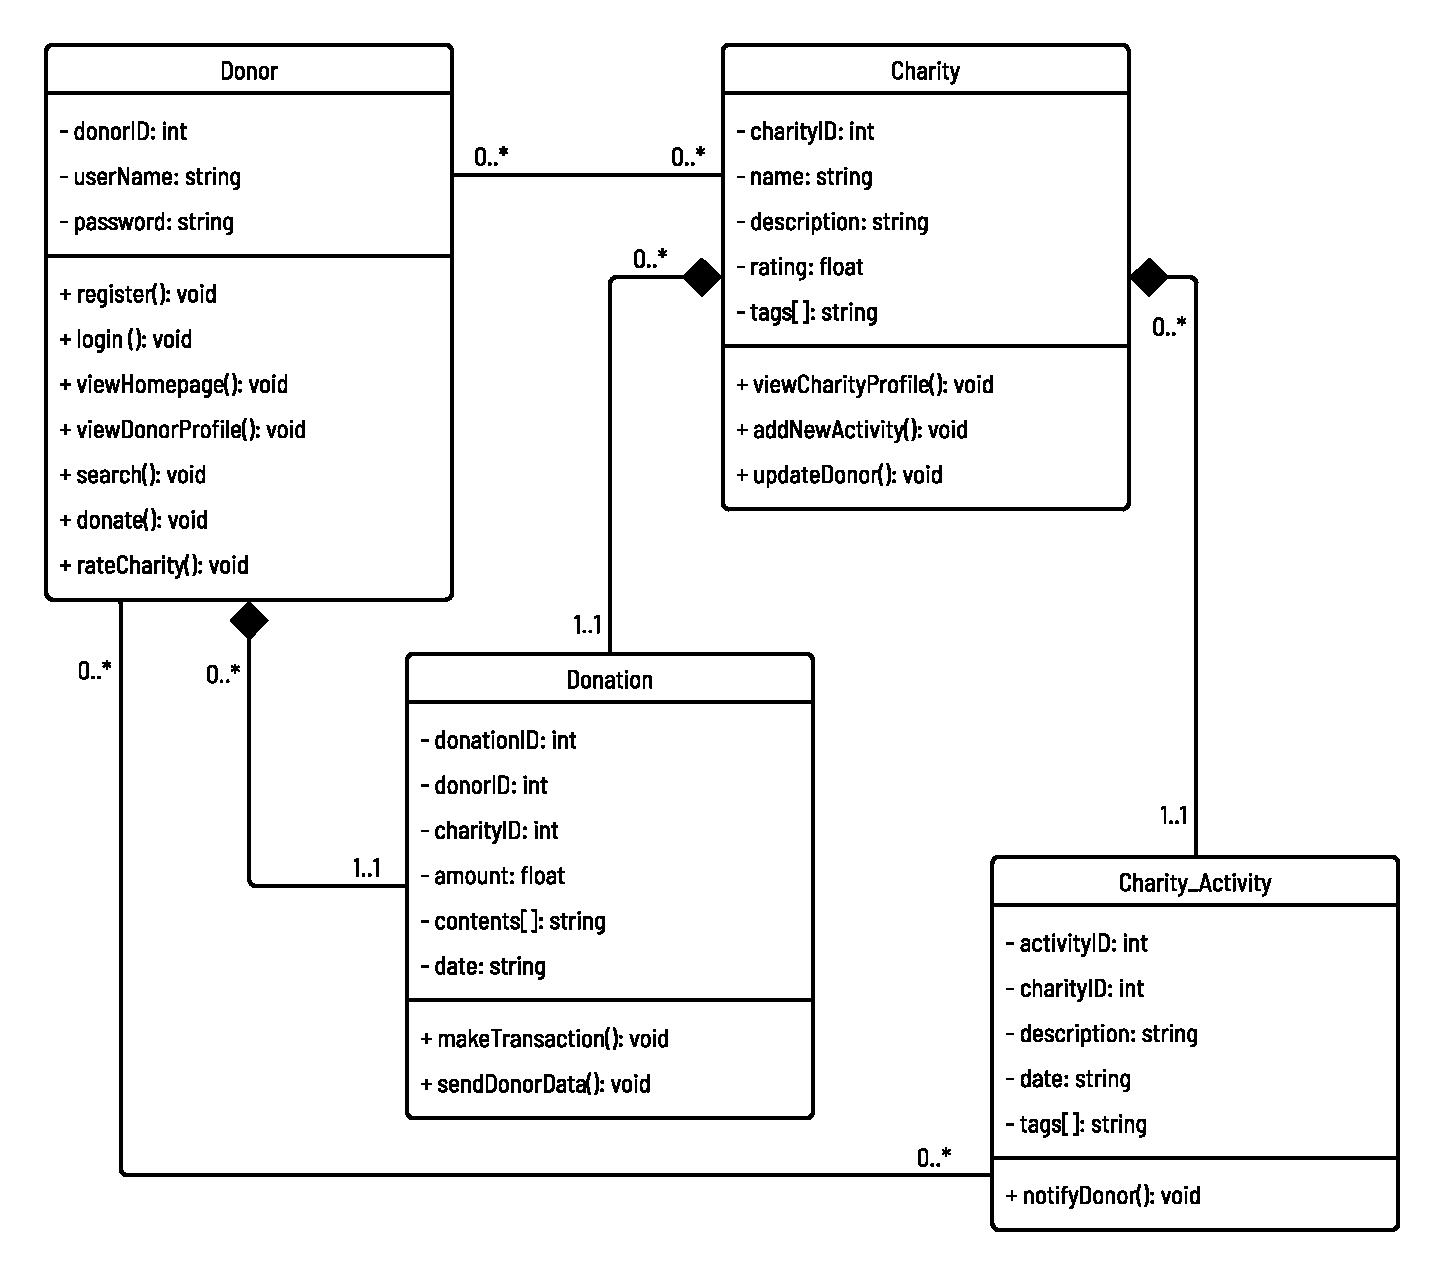
\includegraphics[width=0.75\linewidth]{Class Diagram.png}
    {\caption*{Class Diagram}}
\end{figure}

\addchap{Appendix C: To Be Determined List}

\begin{enumerate}
    \item Details of payment gateway to be used for monetary donations.
\end{enumerate}

\end{document}
